
\begin{figure}[t]
\centering
\definecolor{openarm}{HTML}{2A78D6}
\definecolor{bndarm}{HTML}{C4551F}
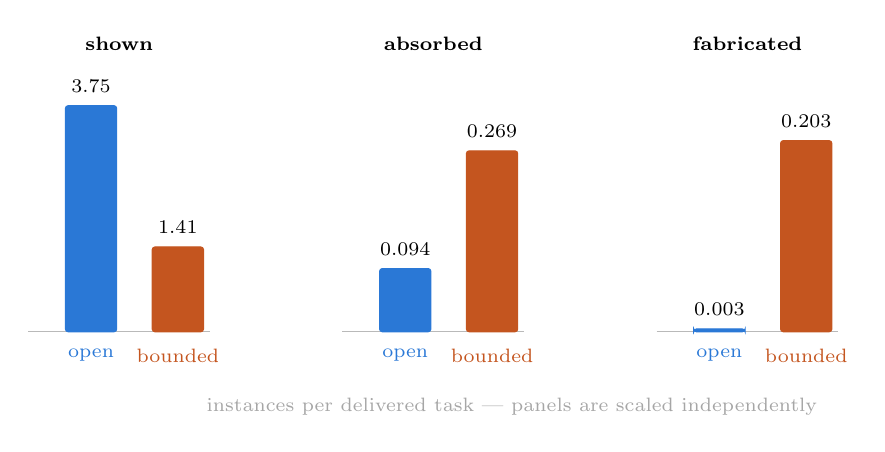
\begin{tikzpicture}[x=1.05cm,y=1.15cm,font=\small]
\node[font=\scriptsize\bfseries,anchor=south] at (0.95,3.00) {shown};
\draw[gray!55] (-0.15,0) -- (2.05,0);
\filldraw[openarm,rounded corners=1pt] (0.30,0) rectangle (0.92,2.497);
\node[font=\scriptsize,anchor=south] at (0.61,2.537) {3.75};
\node[openarm,font=\scriptsize,anchor=north] at (0.61,-0.08) {open};
\filldraw[bndarm,rounded corners=1pt] (1.35,0) rectangle (1.97,0.937);
\node[font=\scriptsize,anchor=south] at (1.66,0.977) {1.41};
\node[bndarm,font=\scriptsize,anchor=north] at (1.66,-0.08) {bounded};
\node[font=\scriptsize\bfseries,anchor=south] at (4.75,3.00) {absorbed};
\draw[gray!55] (3.65,0) -- (5.85,0);
\filldraw[openarm,rounded corners=1pt] (4.10,0) rectangle (4.72,0.698);
\node[font=\scriptsize,anchor=south] at (4.41,0.738) {0.094};
\node[openarm,font=\scriptsize,anchor=north] at (4.41,-0.08) {open};
\filldraw[bndarm,rounded corners=1pt] (5.15,0) rectangle (5.77,1.998);
\node[font=\scriptsize,anchor=south] at (5.46,2.038) {0.269};
\node[bndarm,font=\scriptsize,anchor=north] at (5.46,-0.08) {bounded};
\node[font=\scriptsize\bfseries,anchor=south] at (8.55,3.00) {fabricated};
\draw[gray!55] (7.45,0) -- (9.65,0);
\filldraw[openarm,rounded corners=1pt] (7.90,0) rectangle (8.52,0.031);
\node[font=\scriptsize,anchor=south] at (8.21,0.071) {0.003};
\node[openarm,font=\scriptsize,anchor=north] at (8.21,-0.08) {open};
\filldraw[bndarm,rounded corners=1pt] (8.95,0) rectangle (9.57,2.111);
\node[font=\scriptsize,anchor=south] at (9.26,2.151) {0.203};
\node[bndarm,font=\scriptsize,anchor=north] at (9.26,-0.08) {bounded};
\node[gray!70,font=\scriptsize,anchor=north] at (5.7,-0.62) {instances per delivered task --- panels are scaled independently};
\end{tikzpicture}
\caption{The result nobody designed. A bounded roster is shown roughly a third as much
planted misinformation as an open directory---the filter works---and writes almost three
times as much of it into the deliverable ($+0.175$, CI $[+0.105, +0.242]$). Worse, when it
reaches no one it does not decline to answer: across 287 and 286 delivered tasks the open
arms fabricated a value \emph{once} and the bounded arms 58 times. Filtering bad claims out
before they arrive removes the second source that would have caught them, so the redundancy
argument of \S\ref{sec:framework} shows up here as a failure mode rather than as a benefit.}
\label{fig:credulity}
\end{figure}
